% RiskShip -- informe en formato IEEE (conferencia).
% Compilar con pdfLaTeX:
%   cd informe && Rscript -e 'tinytex::pdflatex("riskship_rna.tex")'
% En Overleaf: subir este archivo y la carpeta figuras/.
% Las figuras las exporta el notebook a informe/figuras/ (300 ppp) en cada
% ejecución completa; no se editan a mano.
%
% Todas las cifras provienen de la ejecución confirmada de
% notebooks/rna_shipment_loss.ipynb (5 semillas, RNA_TIME_LIMIT=600) y están
% registradas en README.md ("Experimental protocol and results"). Si el
% notebook se vuelve a ejecutar y algún número cambia, hay que actualizarlo
% aquí también.
\documentclass[conference]{IEEEtran}

\usepackage[utf8]{inputenc}
\usepackage[T1]{fontenc}
\usepackage[spanish,es-tabla,es-nodecimaldot,es-noshorthands]{babel}
\usepackage{amsmath}
\usepackage{array}
\usepackage{booktabs}
\usepackage{cite}
\usepackage{graphicx}
\usepackage{url}

\graphicspath{{figuras/}}

% Nombres de columnas del conjunto de datos (admite guiones bajos).
\newcommand{\col}[1]{\texttt{\detokenize{#1}}}

\renewcommand{\IEEEkeywordsname}{Palabras clave}

\begin{document}

\title{RiskShip: Priorización Inteligente de Envíos con Riesgo de Falla\\
{\large Solución con redes neuronales}}

\author{\IEEEauthorblockN{Kevin Bueno S. y Lizeth Portela L.}
\IEEEauthorblockA{\textit{Departamento de Ingeniería, Pontificia Universidad Javeriana}\\
Bogotá D.C., Colombia\\
bueno.kevin@javeriana.edu.co, portelali@javeriana.edu.co}}

\maketitle

\begin{abstract}
RiskShip es un agente de priorización que estima el riesgo de pérdida de un
envío en el momento de su creación, antes del despacho, y ordena los casos para
que un equipo con capacidad limitada revise primero los más críticos. Este
informe presenta la solución basada en redes neuronales sobre 262\,317
registros históricos de envíos de Mercado Libre. El aporte central es el
control de la fuga de información: se identificaron y descartaron columnas que
reformulan la etiqueta, una fecha y una taxonomía de regiones que la codifican
de forma silenciosa, y meses cuya etiqueta aún no había madurado. Con una
partición temporal y cinco semillas, el modelo obtiene un PR-AUC de
0,750~$\pm$~0,002 y un ROC-AUC de 0,824~$\pm$~0,002 sobre un mes posterior al
entrenamiento. Proyectado a la prevalencia real de cerca del 0,1\,\%, revisar
el 1\,\% de los envíos capturaría el 30\,\% de las pérdidas, unas 30 veces más
que una revisión al azar.
\end{abstract}

\begin{IEEEkeywords}
redes neuronales, priorización de riesgo, logística, fuga de información,
partición temporal, AutoML
\end{IEEEkeywords}

\section{Introducción}

Las plataformas de comercio electrónico operan redes logísticas en las que un
envío atraviesa centros de \textit{fulfillment}, \textit{cross-docking},
transporte intermedio y última milla~\cite{meli10k}. La capacidad humana de
monitoreo es limitada, de modo que el valor de un modelo no está solo en
clasificar bien, sino en concentrar la atención en la fracción de casos con
mayor riesgo. Las redes neuronales ya se han usado para estimar riesgo de
retraso en cadenas de suministro y mensajería~\cite{bortolini,ye}.

RiskShip se formula como un agente racional: observa los atributos del envío,
estima un puntaje de riesgo entre 0 y 1, ordena los casos y recomienda cuáles
revisar primero; la decisión final sigue siendo humana. Este informe cubre la
primera de las cuatro técnicas previstas en el proyecto, las redes neuronales,
y fija el protocolo experimental que compartirán las demás.

\textbf{Alcance.} La propuesta inicial consideraba envíos en curso, con
variables de trazabilidad hasta un instante de corte, y como falla la pérdida
o el retraso crítico. Esta primera validación se acotó a predecir la
\emph{pérdida} en el \emph{momento de creación del envío}: es el punto donde
una intervención es más barata y, en los datos disponibles, toda la línea de
tiempo de estados es posterior a ese momento.

\section{Datos y control de la fuga de información}

El conjunto de datos unifica exportaciones de envíos de Mercado Libre:
262\,317 filas y 58 columnas, con la etiqueta binaria \col{is_lost} (24,3\,\%
de positivos). Es una muestra de casos y controles: como la pérdida real
ronda el 0,1\,\%, se conservaron las pérdidas y solo una fracción de los envíos
sin pérdida. Cada fila es un \emph{artículo} de un envío, no un envío: hay
cerca de 246\,000 envíos distintos y la etiqueta nunca difiere dentro de uno.
% TODO autores: confirmar aquí la autorización de uso académico de los datos.
Los identificadores de envío y de artículo no se usan como variables.

Como la predicción ocurre en la creación, solo es válida la información
conocida en ese momento. El análisis exploratorio mostró que varias columnas
de apariencia legítima codifican la etiqueta por la forma en que se extrajeron
las dos clases. La Tabla~\ref{tab:limpieza} resume los hallazgos y la decisión
tomada en cada caso.

\begin{table}[htbp]
\caption{Fuentes de fuga de información y decisión de limpieza}
\label{tab:limpieza}
\centering
\footnotesize
\begin{tabular}{>{\raggedright\arraybackslash}p{0.26\linewidth}>{\raggedright\arraybackslash}p{0.38\linewidth}>{\raggedright\arraybackslash}p{0.22\linewidth}}
\toprule
\textbf{Fuente} & \textbf{Evidencia} & \textbf{Decisión}\\
\midrule
Causa, clasificación y reembolso de la pérdida (9 columnas) & No nulas en el 100\,\% de las filas perdidas y en el 0\,\% del resto & Descartar\\
Línea de tiempo de estados & Posterior a la creación del envío & Descartar\\
\col{DATEPARAMETER} & Igual al inicio del envío si no se perdió; unos 9 días posterior si se perdió & Descartar\\
\col{LG_REGION} & La misma instalación recibe nombres de región distintos según la clase & Descartar\\
Nulos en peso, dimensión, valor o cantidad & Cerca del 100\,\% de esas filas están perdidas & Eliminar filas\\
Meses recientes & Tasa de pérdida de 0\,\% a 1,3\,\% frente a 31--47\,\% en los meses previos: la etiqueta aún no madura & Eliminar meses\\
\bottomrule
\end{tabular}
\end{table}

Los meses válidos se calculan a partir de los datos: se conservan aquellos con
ambas clases presentes y se descartan los meses finales cuya tasa de pérdida
es inferior a la mitad de la mediana mensual. No se usa ninguna fecha absoluta
como variable, solo el día de la semana, para que el modelo no reaprenda ese
artefacto. Una auditoría de pureza revisa además, para cada variable
categórica, qué proporción de filas cae en valores con tasa de pérdida extrema.

El conjunto limpio tiene 165\,002 filas (de 2025-09 a 2026-03, 37\,\% de
positivos) y 13 variables: seis categóricas (tipo de \textit{picking},
instalación, dominio, categoría, marca y tipo de voluminoso), seis numéricas
(peso, dimensión máxima, valor, cantidad de artículos, razón de servicio del
mes anterior e indicador de voluminoso) y el día de la semana. La
Fig.~\ref{fig:exploracion} muestra que la tasa de pérdida varía con fuerza
entre instalaciones y poco entre los principales tipos de \textit{picking}.

% ---------------------------------------------------------------------------
% IMAGEN 1 (ancho completo, dos columnas).
% Figura de la sección 4 del notebook con dos paneles,
%   "Tasa de pérdida por tipo de picking" y
%   "Tasa de pérdida por instalación (15 con mayor volumen)".
% Archivo: figuras/tasa_perdida_picking_instalacion.png
% ---------------------------------------------------------------------------
\begin{figure*}[htbp]
\centering
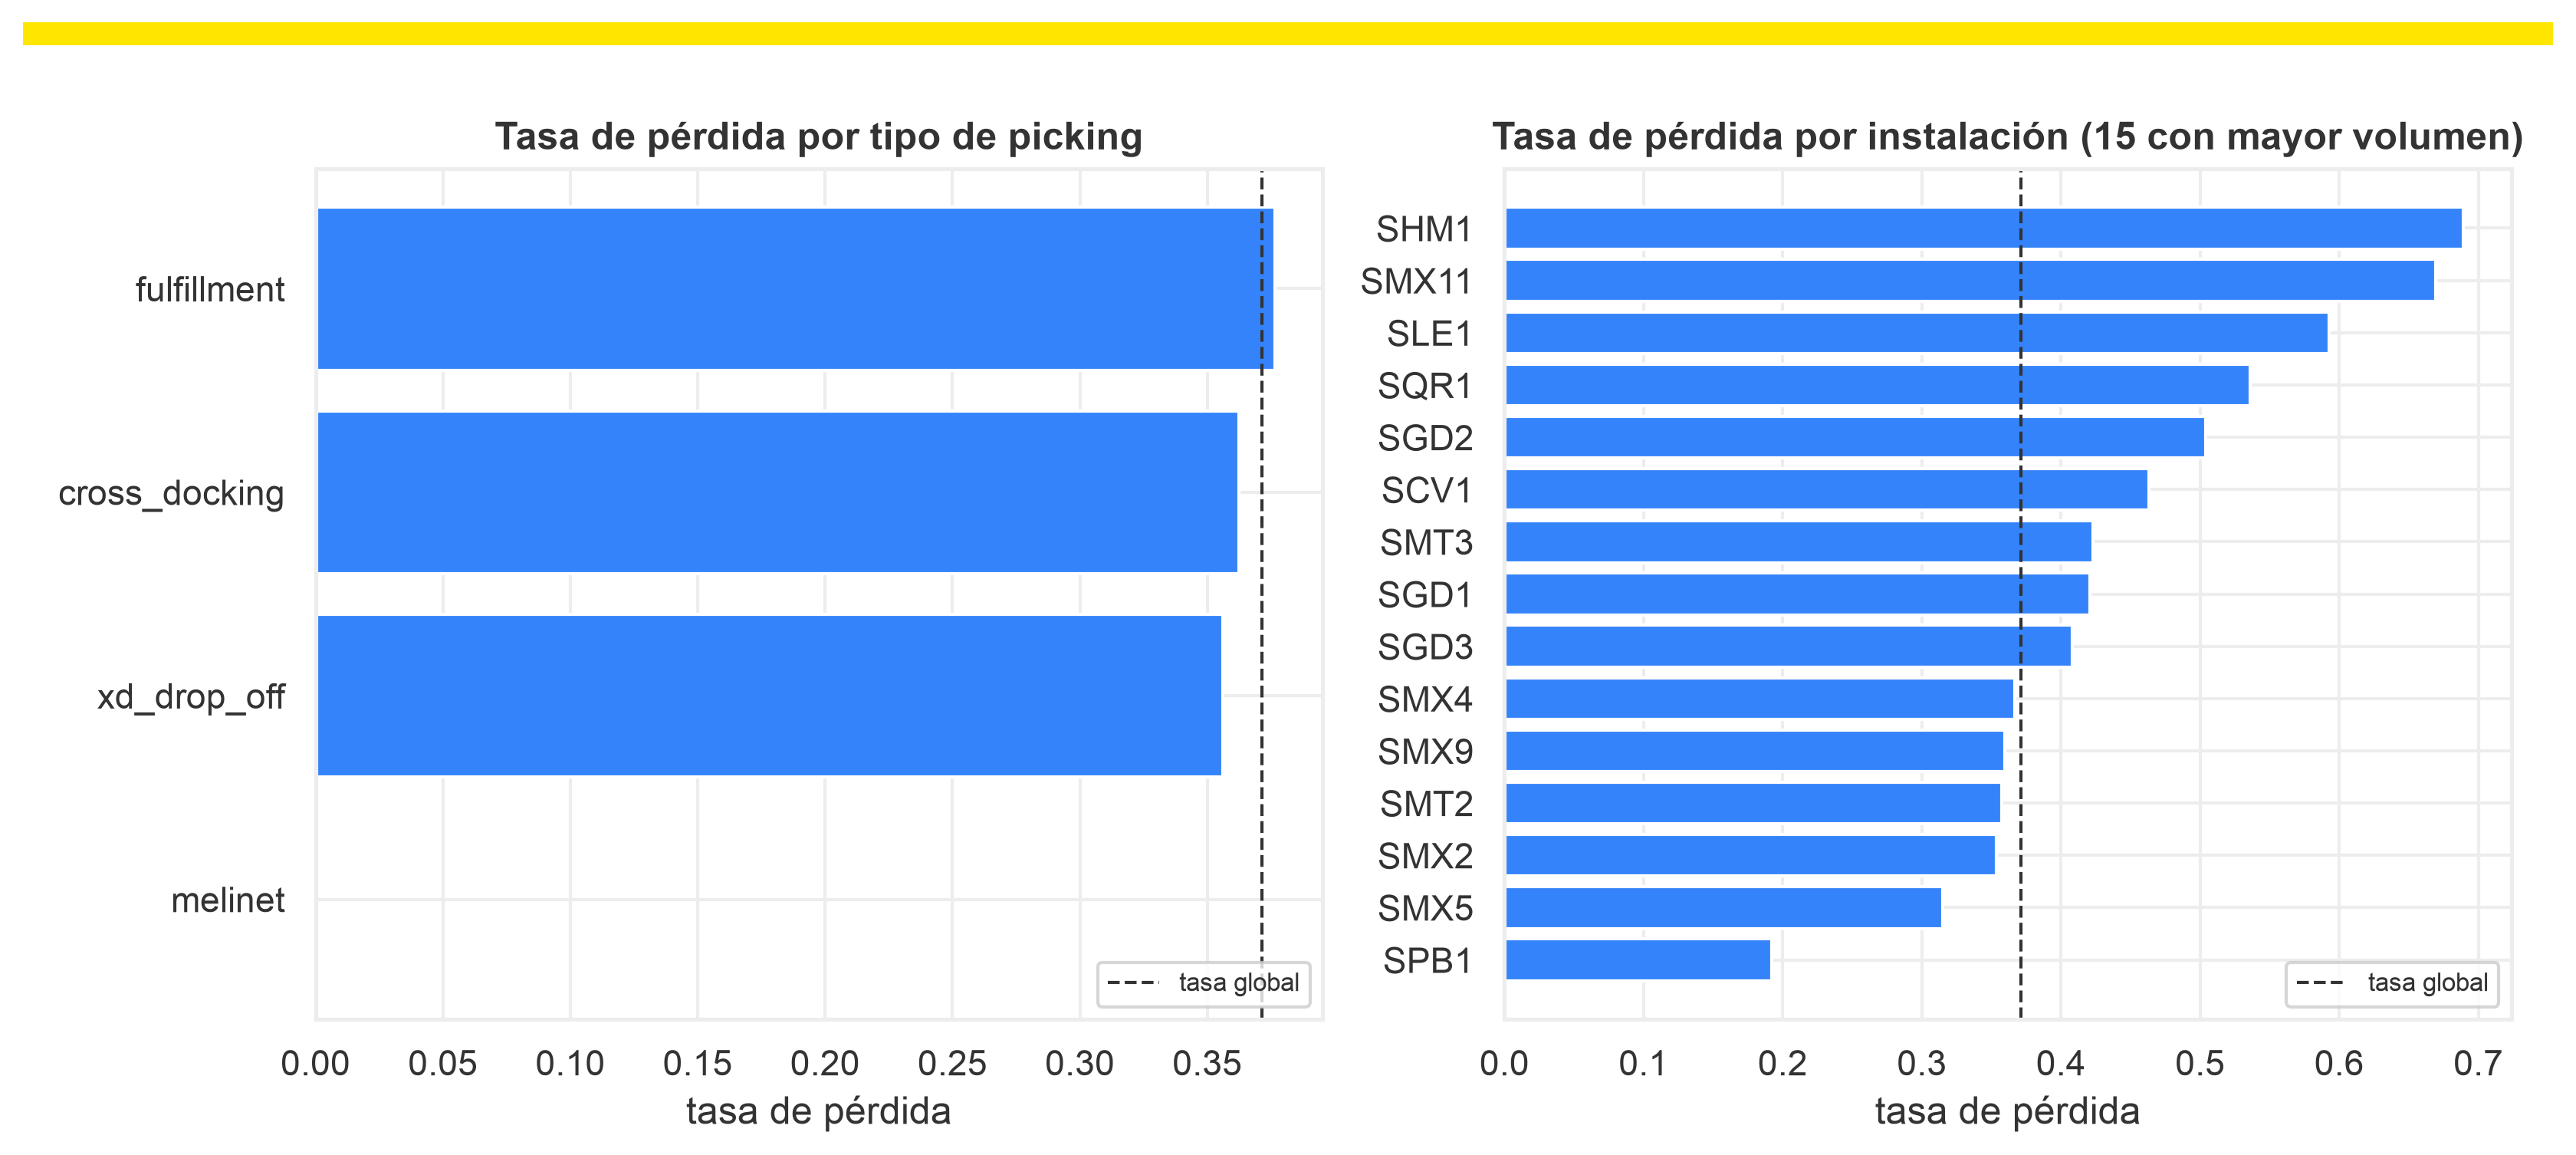
\includegraphics[width=0.85\textwidth]{tasa_perdida_picking_instalacion.png}
\caption{Tasa de pérdida por tipo de \textit{picking} y por instalación
logística en los datos limpios. La línea punteada marca la tasa global.}
\label{fig:exploracion}
\end{figure*}

\section{Metodología}

\subsection{Modelo}

Se usa AutoGluon-Tabular~\cite{autogluon} restringido a sus dos motores de
redes neuronales, sin árboles: un perceptrón multicapa en PyTorch (4 capas de
128 neuronas, ReLU, \textit{dropout} de 0,1, optimizador Adam, tasa
de aprendizaje de $3\times10^{-4}$) y el modelo tabular de fastai (capas de 200
y 100 neuronas, \textit{dropout} de 0,1, tasa de aprendizaje de $10^{-2}$).
Ambos representan las variables categóricas con \textit{embeddings} y se
detienen de forma temprana según la validación. Sus salidas se combinan en un
ensamble ponderado. Se usaron los hiperparámetros por defecto; AutoGluon
gestiona internamente la imputación, la codificación y el escalado.

La métrica optimizada es la precisión promedio (PR-AUC) y no la exactitud, que
resulta engañosa con clases desbalanceadas~\cite{saito}: un modelo que siempre
predijera ``no perdido'' ya acertaría en cerca de dos tercios de los casos.

\subsection{Protocolo experimental}

La partición es temporal (Tabla~\ref{tab:particion}): se entrena con los meses
más antiguos y se valida y se prueba con los más recientes, de modo que
ninguna información futura influye en el entrenamiento. Todas las filas de un
envío comparten fecha de inicio, por lo que ningún envío queda repartido entre
particiones; el notebook lo verifica.

\begin{table}[htbp]
\caption{Partición temporal de los datos limpios}
\label{tab:particion}
\centering
\footnotesize
\begin{tabular}{lcrrr}
\toprule
\textbf{Partición} & \textbf{Meses} & \textbf{Filas} & \textbf{Envíos} & \textbf{Positivos}\\
\midrule
Entrenamiento & 2025-09 a 2026-01 & 125\,082 & 112\,303 & 39,0\,\%\\
Validación & 2026-02 & 18\,831 & 17\,297 & 31,6\,\%\\
Prueba & 2026-03 & 21\,089 & 19\,506 & 31,2\,\%\\
\bottomrule
\end{tabular}
\end{table}

El entrenamiento se repite con cinco semillas (42 a 46). La partición y el
conjunto de prueba son idénticos en todas las corridas; solo cambia el
entrenamiento de las redes (inicialización de pesos, orden de los lotes y
\textit{dropout}). Se reportan la media y la desviación estándar muestral. El
análisis detallado usa la semilla con mejor PR-AUC en \emph{validación}, nunca
en prueba.

Además de PR-AUC, ROC-AUC, exhaustividad (\textit{recall}), precisión y F1 de
la clase ``perdido'' con umbral 0,5, se miden Recall@$K$ y Precision@$K$: al
revisar solo el $K$\,\% de los envíos con mayor puntaje, qué proporción de las
pérdidas reales queda dentro de ese grupo y qué proporción de lo revisado era
realmente una pérdida.

\section{Resultados}

La Tabla~\ref{tab:metricas} muestra el desempeño sobre el mes de prueba. La
referencia de PR-AUC para un orden aleatorio es la tasa de positivos, 0,312.
La dispersión entre semillas es mínima, por lo que el resultado no depende de
la semilla. Cada semilla se entrena en unos 100~s. En el modelo de referencia
(semilla 46) la red de fastai alcanza un PR-AUC de 0,733, la de PyTorch 0,680
y el ensamble 0,749. Su matriz de confusión tiene 13\,425 verdaderos
negativos, 1\,082 falsos positivos, 3\,094 falsos negativos y 3\,488 verdaderos
positivos. La Fig.~\ref{fig:pr} muestra su curva de precisión-exhaustividad.

\begin{table}[htbp]
\caption{Métricas en el conjunto de prueba (cinco semillas)}
\label{tab:metricas}
\centering
\footnotesize
\begin{tabular}{lc}
\toprule
\textbf{Métrica} & \textbf{Media $\pm$ desviación}\\
\midrule
PR-AUC & 0,7496 $\pm$ 0,0020\\
ROC-AUC & 0,8241 $\pm$ 0,0020\\
Exhaustividad (umbral 0,5) & 0,5339 $\pm$ 0,0136\\
Precisión (umbral 0,5) & 0,7568 $\pm$ 0,0157\\
F1 (umbral 0,5) & 0,6259 $\pm$ 0,0044\\
Tasa de falsos positivos (umbral 0,5) & 0,0781 $\pm$ 0,0089\\
PR-AUC en validación & 0,7644 $\pm$ 0,0019\\
\bottomrule
\end{tabular}
\end{table}

% ---------------------------------------------------------------------------
% IMAGEN 2 (una columna).
% Figura de la sección 7 del notebook titulada
%   "Curva de precisión-exhaustividad (AP = 0.749)".
% Archivo: figuras/curva_precision_exhaustividad.png
% ---------------------------------------------------------------------------
\begin{figure}[htbp]
\centering
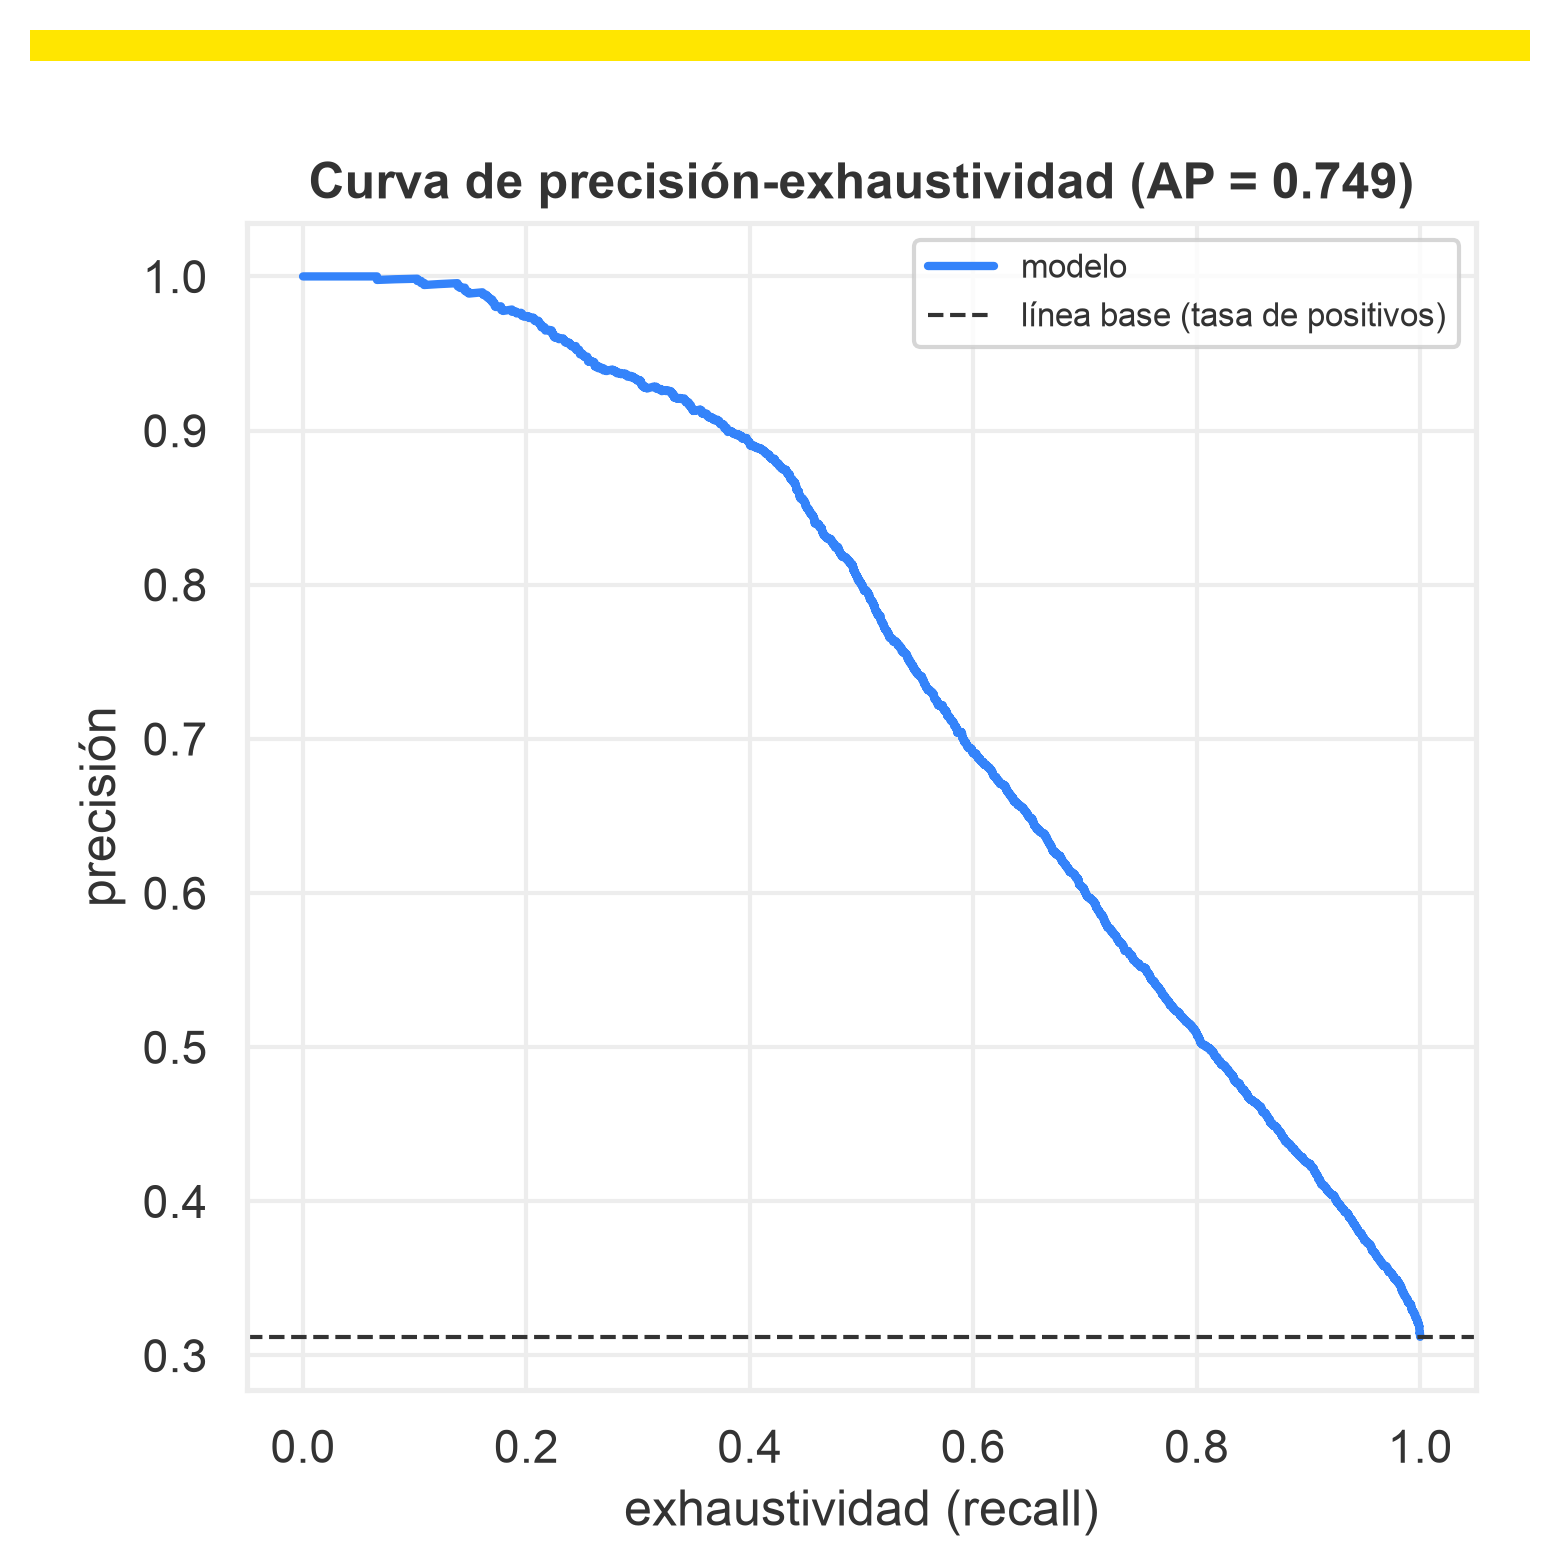
\includegraphics[width=0.85\linewidth]{curva_precision_exhaustividad.png}
\caption{Curva de precisión-exhaustividad del modelo de referencia en el
conjunto de prueba. La línea punteada es la tasa de positivos.}
\label{fig:pr}
\end{figure}

\subsection{Calidad de la priorización}

La Tabla~\ref{tab:ranking} mide la calidad del orden dentro de la muestra. Con alrededor de un
tercio de positivos, ni un orden perfecto captura más de $K/0{,}312$ de las
pérdidas al revisar el $K$\,\%; el modelo queda cerca de ese techo hasta el
10\,\% revisado (Fig.~\ref{fig:ganancia}).

\begin{table}[htbp]
\caption{Métricas de priorización en prueba (cinco semillas)}
\label{tab:ranking}
\centering
\footnotesize
\begin{tabular}{rrccc}
\toprule
\textbf{$K$} & \textbf{Filas} & \textbf{Recall@$K$} & \textbf{Techo} & \textbf{Precision@$K$}\\
\midrule
1\,\% & 211 & 0,032 $\pm$ 0,000 & 0,032 & 1,000 $\pm$ 0,000\\
5\,\% & 1\,054 & 0,158 $\pm$ 0,001 & 0,160 & 0,987 $\pm$ 0,004\\
10\,\% & 2\,109 & 0,302 $\pm$ 0,002 & 0,320 & 0,942 $\pm$ 0,006\\
20\,\% & 4\,218 & 0,506 $\pm$ 0,002 & 0,641 & 0,790 $\pm$ 0,004\\
\bottomrule
\end{tabular}
\end{table}

% ---------------------------------------------------------------------------
% IMAGEN 3 (una columna).
% Figura de la sección 7 del notebook titulada
%   "Pérdidas capturadas según la fracción revisada"
%   (curva de ganancia acumulada con las etiquetas 3%, 16%, 30% y 51%).
% Archivo: figuras/curva_ganancia.png
% ---------------------------------------------------------------------------
\begin{figure}[htbp]
\centering
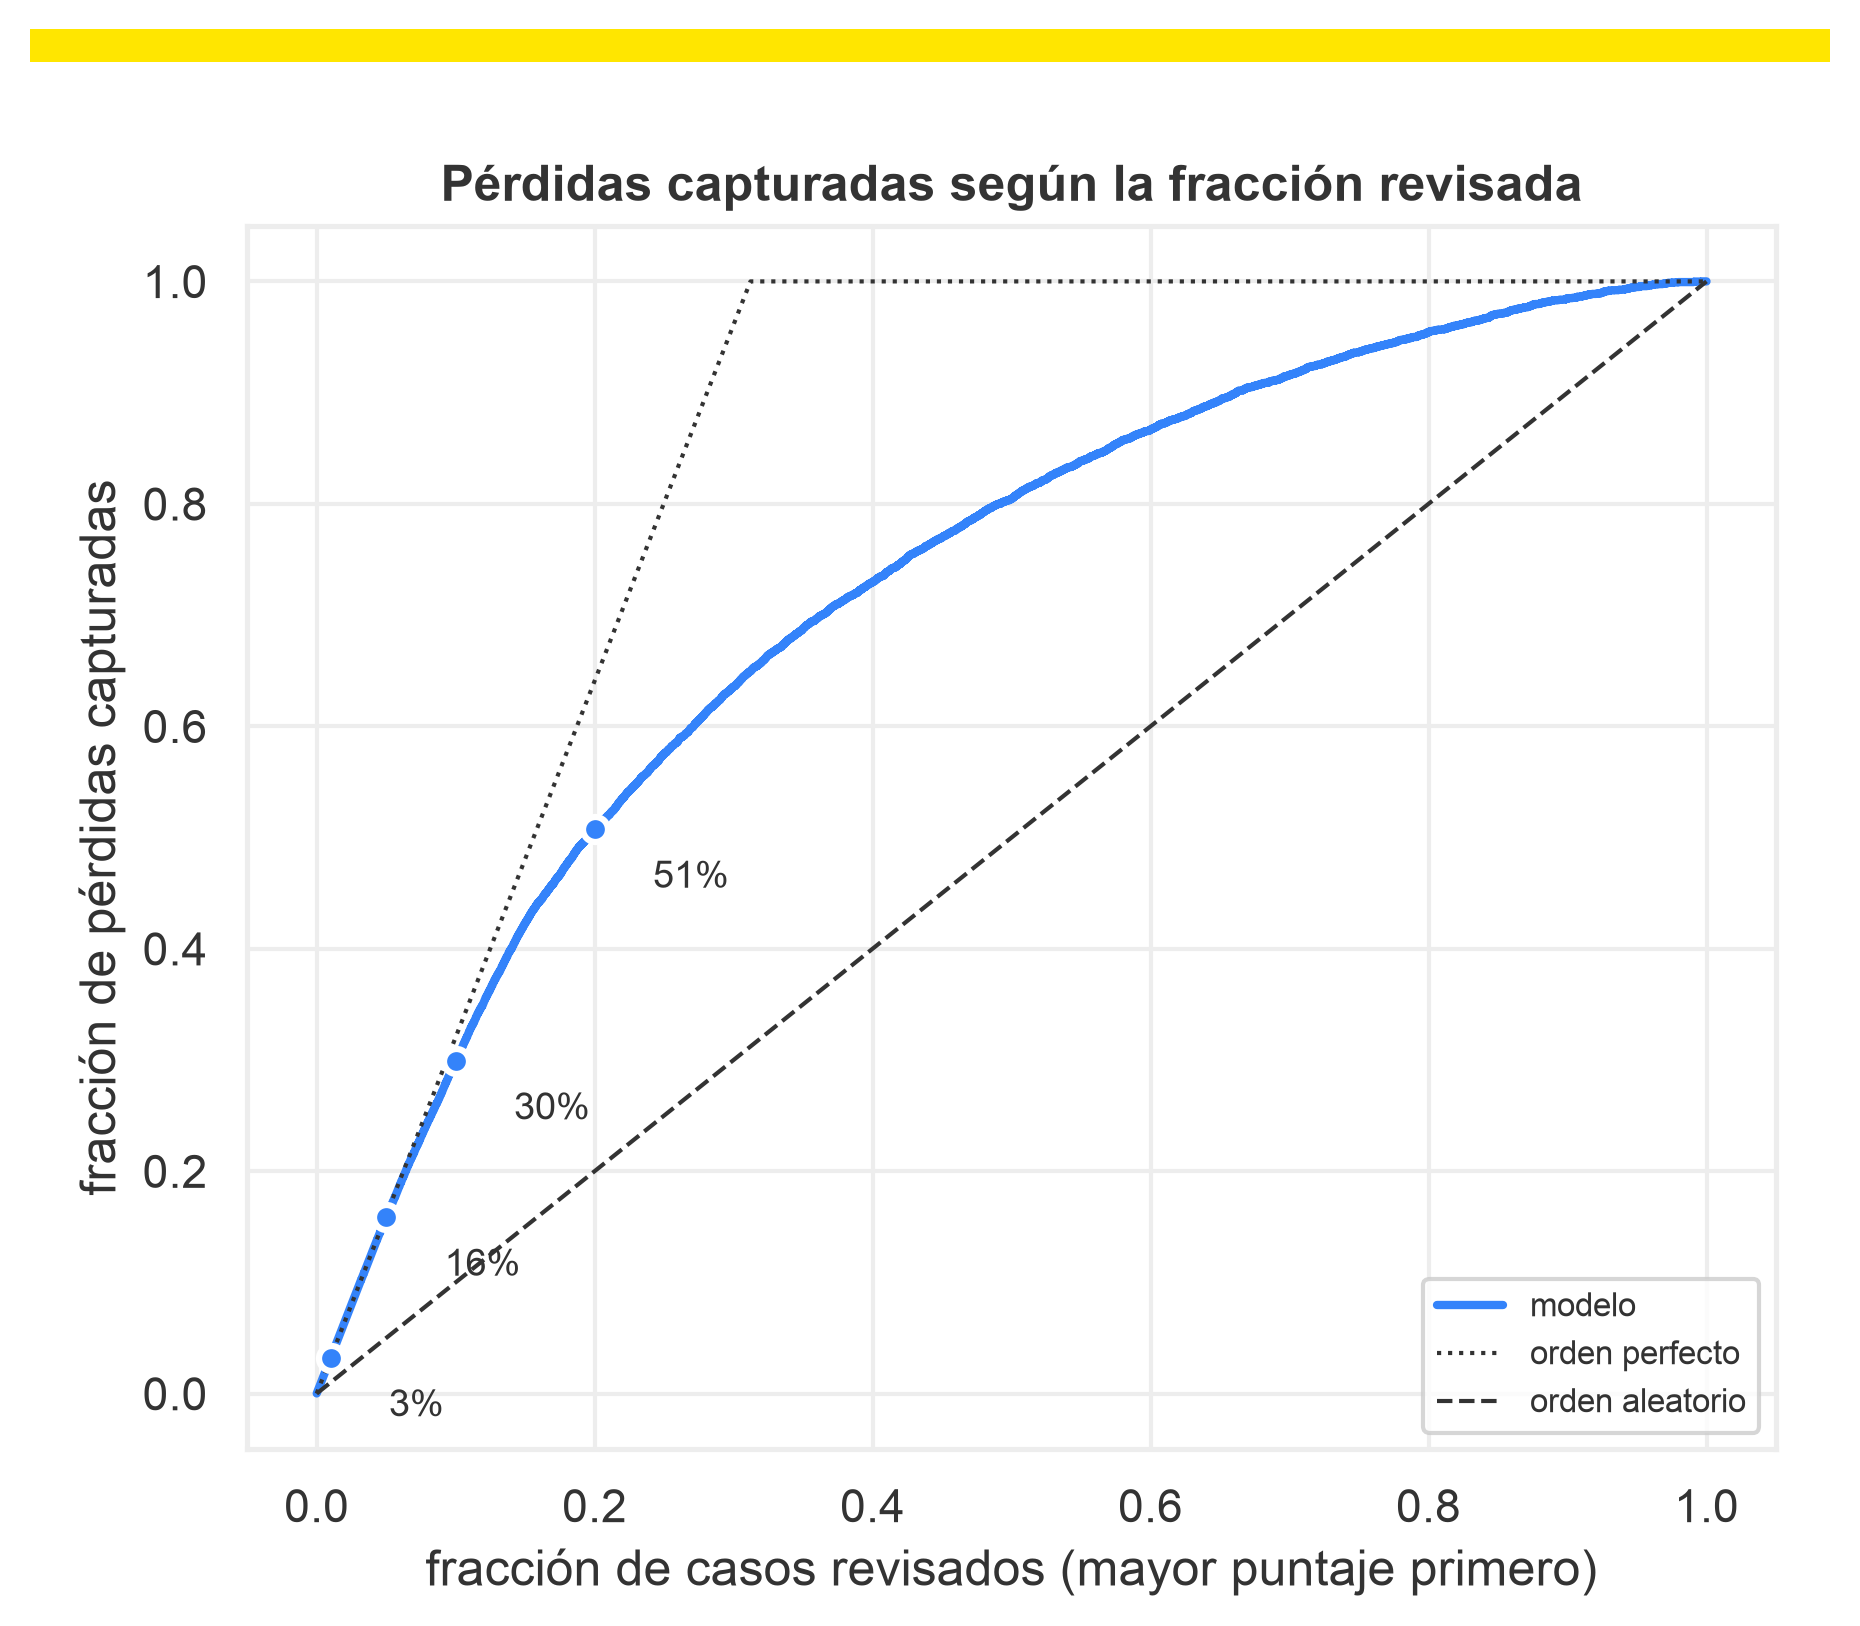
\includegraphics[width=\linewidth]{curva_ganancia.png}
\caption{Fracción de pérdidas capturadas según la fracción de casos
revisados, frente al orden aleatorio y al orden perfecto.}
\label{fig:ganancia}
\end{figure}

\subsection{Proyección a la prevalencia real}

Las Tablas~\ref{tab:metricas} y~\ref{tab:ranking} describen el desempeño
\emph{dentro de la muestra}. En un diseño de casos y controles solo la
exhaustividad y la tasa de falsos positivos (TFP) se trasladan sin cambios a
la operación, porque cada una se calcula dentro de una sola clase; por eso el
ROC-AUC es válido tal cual, mientras que la precisión, el PR-AUC y las
métricas en $K$ dependen de la prevalencia. Con prevalencia real $\pi$, para
cualquier umbral:
\begin{equation}
f = \pi\, r + (1-\pi)\,\mathrm{TFP}, \qquad p = \frac{\pi\, r}{f},
\end{equation}
donde $r$ es la exhaustividad, $f$ la fracción de envíos revisados y $p$ la
precisión. La Tabla~\ref{tab:proyeccion} aplica la conversión al modelo de
referencia con $\pi = 0{,}001$. Con puntaje mínimo de 0,78 se revisaría el
1\,\% de los envíos y se capturaría el 30\,\% de las pérdidas: una pérdida
por cada 33 envíos revisados, 30 veces mejor que al azar. La proyección supone
que los negativos de la muestra representan a los reales, y $\pi$ es una
estimación del equipo, no un dato medido.

\begin{table}[htbp]
\caption{Proyección a una prevalencia real de 0,1\,\% (modelo de referencia)}
\label{tab:proyeccion}
\centering
\footnotesize
\setlength{\tabcolsep}{3.5pt}
\begin{tabular}{cccccc}
\toprule
\textbf{Puntaje} & & & \textbf{Envíos} & \textbf{Revisados} & \textbf{Mejora}\\
\textbf{mínimo} & \textbf{Exhaust.} & \textbf{TFP} & \textbf{revisados} & \textbf{por pérdida} & \textbf{sobre azar}\\
\midrule
0,91 & 0,159 & 0,0008 & 0,09\,\% & 6 & 173\\
0,78 & 0,299 & 0,0097 & 1,00\,\% & 33 & 30\\
0,53 & 0,507 & 0,0606 & 6,10\,\% & 120 & 8,3\\
0,50 & 0,530 & 0,0746 & 7,50\,\% & 142 & 7,1\\
\bottomrule
\end{tabular}
\end{table}

\subsection{Importancia de variables}

La Tabla~\ref{tab:importancia} muestra la importancia por permutación: la
caída de PR-AUC al desordenar cada variable. Las variables restantes aportan
menos de 0,005.

\begin{table}[htbp]
\caption{Importancia por permutación (modelo de referencia)}
\label{tab:importancia}
\centering
\footnotesize
\begin{tabular}{lc}
\toprule
\textbf{Variable} & \textbf{Caída de PR-AUC}\\
\midrule
\col{DOM_DOMAIN_ID} (dominio del producto) & 0,197\\
\col{CANTIDAD_ITEMS} & 0,144\\
\col{SHP_LG_FACILITY_ID} (instalación) & 0,070\\
\col{PESO_TOTAL_KG} & 0,068\\
\col{ORD_CATEGORY_NAME_L1} (categoría) & 0,038\\
\col{BRAND_NAME} (marca) & 0,018\\
\col{PICKING_TYPE} & 0,017\\
\bottomrule
\end{tabular}
\end{table}

\section{Discusión y limitaciones}

\textbf{El muestreo es válido; la extracción por clase, no.} Sobrerrepresentar
las pérdidas es la práctica estándar ante un evento del 0,1\,\%. Los artefactos
de la Tabla~\ref{tab:limpieza} no vienen de esa proporción, sino de que las dos
clases se extrajeron por caminos distintos. Una nueva extracción debería usar
una sola consulta para ambas clases (misma población, filtros, tablas y ventana
de fechas de creación), submuestrear al azar solo los negativos con una tasa
registrada, incluir únicamente envíos con la etiqueta ya madura y tomar los
atributos como estaban al crear el envío. Sin la tasa de muestreo, las
probabilidades predichas no se pueden calibrar: sirven para ordenar, no como
probabilidad de pérdida. Como la muestra ya tiene un tercio de positivos, no se
aplicó ponderación de clases ni remuestreo.

\textbf{Posible fuga residual en el dominio del producto.} Precision@1\,\% es
exactamente 1,0 en las cinco semillas, y los umbrales más altos de la
Tabla~\ref{tab:proyeccion} dependen de una TFP casi nula. Seis valores de \col{DOM_DOMAIN_ID}
tienen 100\,\% de pérdida con 200 a 834 filas cada uno, y esa es la variable
más importante del modelo. El patrón coincide con el artefacto de taxonomía
hallado en \col{LG_REGION} y probablemente infla el tope del orden. Debe
investigarse antes de tomar esa precisión como señal real.

\textbf{Costo de una evaluación honesta.} Una versión previa, con partición
aleatoria y un mes de etiqueta inmadura, obtenía ROC-AUC de 0,848 y PR-AUC de
0,800. La caída a 0,824 y 0,750 es el precio de evaluar sobre envíos
posteriores al entrenamiento, no un retroceso del modelo.

\textbf{Otras limitaciones.} El conjunto de prueba cubre un solo mes, así que
mide la generalización al mes siguiente y no entre temporadas. Las métricas
están a nivel de artículo, no de envío. No se exploraron de forma explícita
capas, neuronas, activación ni regularización. Las semillas miden el ruido de
entrenamiento, no la sensibilidad a la ventana temporal.

\textbf{Consideraciones éticas.} El puntaje puede reflejar sesgos históricos
hacia ciertas instalaciones o categorías; expresa correlación, no causalidad,
y se plantea como apoyo a la priorización humana, nunca como mecanismo
automático de sanción.

\section{Conclusiones y trabajo futuro}

Una red neuronal entrenada solo con información disponible en la creación del
envío ordena el riesgo de pérdida de forma útil y estable: en un mes no visto,
y proyectado a la prevalencia real, revisar el 1\,\% de los envíos capturaría
cerca del 30\,\% de las pérdidas. El
resultado más valioso del trabajo no es la métrica, sino el control de la fuga
de información: sin él, el modelo habría reportado un desempeño casi perfecto
aprendiendo artefactos de la extracción.

El trabajo inmediato es auditar \col{DOM_DOMAIN_ID}, explorar los
hiperparámetros de la red y agregar las métricas a nivel de envío. El mismo
protocolo (partición temporal, conjunto de prueba, semillas y métricas de
priorización) se aplicará a las técnicas restantes del proyecto: reglas
evolucionadas con algoritmo genético, inferencia difusa y métodos de ensamble,
para comparar desempeño, interpretabilidad y costo computacional.

\begin{thebibliography}{00}
\bibitem{meli10k} MercadoLibre, Inc., ``Annual Report on Form 10-K for the
fiscal year ended December 31, 2025,'' U.S. Securities and Exchange
Commission, feb. 2026.
\bibitem{bortolini} M. Bortolini \textit{et al.}, ``A deep learning approach to
predict supply chain delivery delay risk based on macroeconomic indicators: A
case study in the automotive sector,'' \textit{Applied Sciences}, vol. 14,
no. 11, art. 4688, 2024, doi: 10.3390/app14114688.
\bibitem{ye} B. Ye, J. Zuo, X. Zhao y L. Luo, ``Research on the express
delivery delay prediction based on neural network in the background of big
data,'' en \textit{Proc. 6th Int. Conf. Electronic, Mechanical, Information
and Management Society}, 2016, pp. 1449--1454, doi: 10.2991/emim-16.2016.294.
\bibitem{autogluon} N. Erickson \textit{et al.}, ``AutoGluon-Tabular: Robust
and accurate AutoML for structured data,'' arXiv:2003.06505, 2020.
\bibitem{saito} T. Saito y M. Rehmsmeier, ``The precision-recall plot is more
informative than the ROC plot when evaluating binary classifiers on imbalanced
datasets,'' \textit{PLoS ONE}, vol. 10, no. 3, art. e0118432, 2015.
\end{thebibliography}

\end{document}
